\documentclass[9pt]{beamer}

\usepackage[T1]{fontenc}
\usepackage[utf8]{inputenc}
\usepackage[frenchb]{babel}
\usepackage{eurosym}

\usepackage{multirow}

\usepackage{graphicx}


\newcommand\host{{\it host} }
\newcommand\device{{\it device} }


% --------- BEGIN STYLE BEAMER ---------
\usetheme{Madrid}
\definecolor{ECNBleu}{HTML}{102648}
\definecolor{ECNJaune}{HTML}{FAB600}

\setbeamercolor{frametitle}{bg=ECNBleu,fg=white} %le titre de la frame, en haut
\setbeamercolor{title in head/foot}{bg=ECNJaune,fg=ECNBleu} %barre bas, milieu
\setbeamercolor{author in head/foot}{bg=ECNBleu,fg=ECNJaune} %barre bas, gauche
\setbeamercolor{date in head/foot}{bg=ECNBleu,fg=ECNJaune} %barre bas, droit
\setbeamercolor{section in head/foot}{bg=ECNJaune,fg=ECNBleu} %haut gauche
\setbeamercolor{subsection in head/foot}{bg=ECNBleu,fg=ECNBleu} %haut droite
\setbeamercolor{title}{bg=ECNBleu,fg=white}
\setbeamercolor{block title}{fg=white,bg=ECNBleu}

%\setbeamercolor{normal text}{bg=IUTBleuFonce} %texte
\setbeamercolor{item}{bg=ECNBleu}
\setbeamercolor{subitem}{bg=ECNJaune}
\setbeamercolor{description item}{fg=couleurEmph}
\setbeamercolor{section in toc}{fg=ECNBleu}
%\setbeamercolor{subsubitem}{bg=IUTBleuFonce}

%structure (eq emph dans beamer)
\setbeamercolor{emph}{fg=couleurEmph}
% ----------------------------

\usepackage{listings}

\lstdefinestyle{customc}{
  belowcaptionskip=1\baselineskip,
  breaklines=true,
  frame=L,
  xleftmargin=\parindent,
  language=C,
  showstringspaces=false,
  basicstyle=\tiny\ttfamily,
  keywordstyle=\bfseries\color{green!40!black},
  commentstyle=\itshape\color{purple!40!black},
  identifierstyle=\color{blue},
  stringstyle=\color{orange},
}

\lstset{escapechar=@,style=customc}

\newenvironment<>{questionblock}[1]{%
\setbeamercolor{block title}{bg=ECNJaune,fg=ECNBleu}%
\begin{block}#2{#1}}{\end{block}}

\title[GPGPU]{Programmation sur Processeur Graphique}

\subtitle[\ldots]{
---\\Partie 10 : Instructions atomiques}
\author[P.-E. Hladik]{Pierre-Emmanuel Hladik\\\tiny pierre-emmanuel.hladik@ec-nantes.fr}
\institute[Centrale Nantes]{}
\date{\today}

\begin{document}

\frame{\titlepage}

%%%%%%%%%%%%%%%%%%%%%%%%%%
\begin{frame}[plain]
\frametitle{Calcul d'un histogramme}
      \centering
      \begin{block}{Principe}
	Chaque élément dans un ensemble de données est associé à un "conteneur".

	Exemple :
      	\begin{itemize}
		\item Conteneurs : sections de 4 lettres de l'alphabet : a-d, e-h, i-l,...
		\item Pour chaque caractère d'une chaîne, on incrémente le compteur du conteneur correspondant
		\item Dans la phrase "When nine hundred years old you reach, look as good you will not" on obtient :
	\end{itemize}
	\begin{center}
	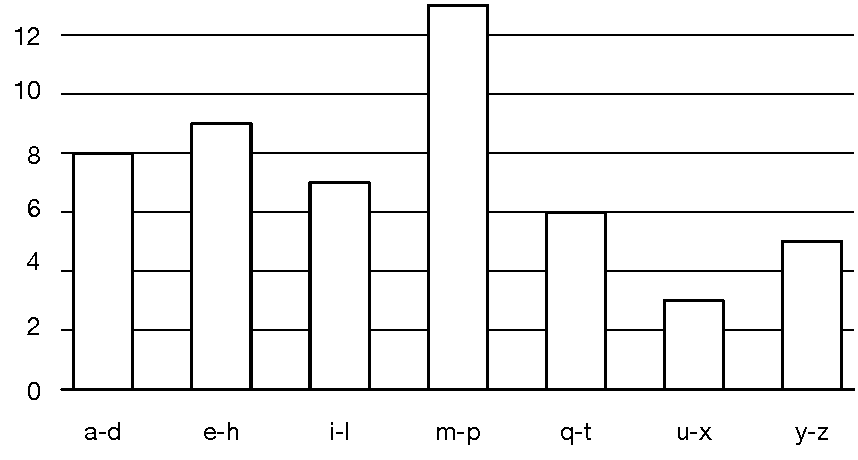
\includegraphics[scale=0.4]{./figures-pdf/histo}
\end{center}
	\end{block}  
\end{frame}
%%%%%%%%%%%%%%%%%%%%%%%%%%
\begin{frame}[plain]
\frametitle{Algorithme parallèle simple : histogramme}
      \centering
      \begin{block}{}
      	\begin{itemize}
		\item Les entrées sont divisées en sections
		\item Chaque thread prend une section comme entrée
		\item Chaque thread itère dans sa section
		\item Pour chaque lettre le compteur de conteneur est incrémenté
	\end{itemize}
	\begin{center}
	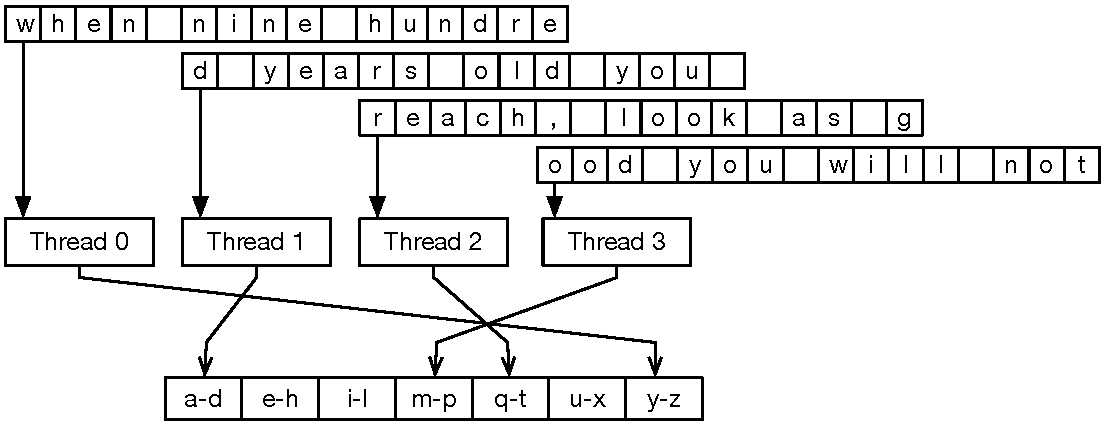
\includegraphics[scale=0.5]{./figures-pdf/algo}
\end{center}
	\end{block}  
\end{frame}
%%%%%%%%%%%%%%%%%%%%%%%%%%
\begin{frame}[plain]
\frametitle{Remarque : accès mémoire sous-optimale}
      \centering
      \begin{block}{}
      	Le découpage par sections entraîne une faible efficacité d'accès à la mémoire
      	\begin{itemize}	
	\item Les threads n'accèdent pas à des données adjacentes
	\item les accès ne sont pas regroupés (coalesced)
	\item La bande passante des DRAM est sous-utilisée
	\end{itemize}
	\begin{center}
	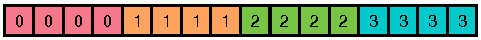
\includegraphics[scale=0.8]{./figures-pdf/uncoalesced}
\end{center}
	\end{block}  
	      \begin{block}{}
      	Optimisation : entrelacer les sections
      	\begin{itemize}	
	\item Les threads procèdent par sections contiguës 
	\item les accès sont ainsi regroupés (coalesced)
	\end{itemize}
	\begin{center}
	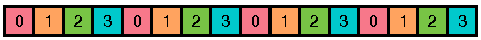
\includegraphics[scale=0.8]{./figures-pdf/coaslesced}
\end{center}
	\end{block}  
\end{frame}
%%%%%%%%%%%%%%%%%%%%%%%%%%
\begin{frame}[plain]
\frametitle{Solution plus optimale : entrelacement des sections}

      \centering
      \begin{block}{}
      	\begin{itemize}
		\item Les entrées sont divisées en sections
		\item Chaque thread prend une section comme entrée
		\item Chaque thread itère dans sa section
		\item Pour chaque lettre le compteur de conteneur est incrémenté
	\end{itemize}
	\begin{center}
	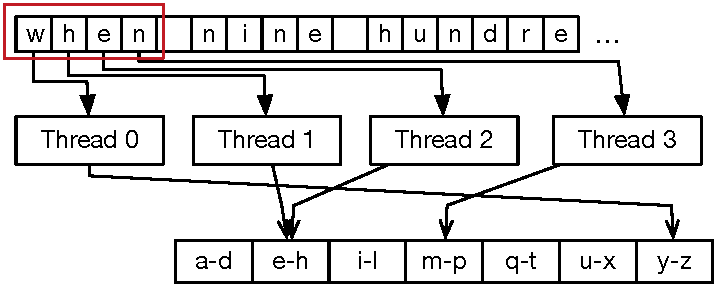
\includegraphics[scale=0.7]{./figures-pdf/algo_coalesced}
\end{center}
	\end{block}  
\end{frame}
%%%%%%%%%%%%%%%%%%%%%%%%%%
\begin{frame}[plain]
\frametitle{Accès concurrent}

      \centering
      \begin{block}{}
      	La mise à jour des compteurs se fait en trois étapes :
	\begin{enumerate}
		\item old <- Mem[x]
		\item new <- old + 1
		\item Mem[x] <- new
	\end{enumerate}
	Il peut y donc y avoir une incohérence dû à l'accès concurrent des threads (dans des warps différents).
	
	{\bf \center  \color{red} Remarque : la notion d'accès concurrent est quelque chose de très classique en programmation concurrente}
	
	\only<2>{\begin{table}[htdp]
	\begin{center}
		\begin{tabular}{|c|l|l|}
		\hline
		Instant & Thread 0 & Thread 32\\
		\hline\hline
		1 & (0) old <- Mem[x] & \\
		\hline
		2 & (1) new <- old + 1 & \\
		\hline
		3 & (1)  Mem[x] <- new & \\
		\hline
		4 & &(1) old <- Mem[x] \\
		\hline
		5 & &(2) new <- old + 1  \\
		\hline
		6 & &(2) Mem[x] <- new  \\
		\hline
		\end{tabular}
	\end{center}
	\end{table}
	}
	\only<3>{\begin{table}[htdp]
	\begin{center}
		\begin{tabular}{|c|l|l|}
		\hline
		Instant & Thread 0 & Thread 32\\
		\hline\hline
		1 & (0) old <- Mem[x] & \\
		\hline
		2 & (1) new <- old + 1 & \\
		\hline
		4 & &(0) old <- Mem[x] \\
		\hline
		3 & (1)  Mem[x] <- new & \\
		\hline
		5 & &(1) new <- old + 1  \\
		\hline
		6 & &(1) Mem[x] <- new  \\
		\hline
		\end{tabular}
	\end{center}
	\end{table}
	}

	\end{block}  
\end{frame}
%%%%%%%%%%%%%%%%%%%%%%%%%%
\begin{frame}[plain]
\frametitle{Principe des opérations atomiques}
      \centering
      \begin{block}{}
      	\begin{itemize}	
	\item Une opération de lecture-modification-écriture est réalisée en une seule instruction matérielle 
	\medskip
	\item Le matériel garantit qu'aucun autre thread ne peut effectuer une autre opération de lecture-écriture sur le même emplacement jusqu'à ce que l'opération atomique en cours soit terminée.
      	\begin{itemize}	
		\item Tout autre thread qui tente d'effectuer une opération atomique au même endroit sera placé dans une file d'attente
		\item Tous les threads effectuent leurs opérations atomiques en {\bf série} pour une même adresse mémoire
	\end{itemize}
	\end{itemize}
	\end{block}  
\end{frame}
%%%%%%%%%%%%%%%%%%%%%%%%%%
\begin{frame}[plain]
\frametitle{Opérations arithmétiques atomiques en CUDA}
      \centering
      \begin{block}{}
      	\begin{itemize}	
		\item Effectuées par l'appel de fonctions qui sont traduites en une unique instruction :
		      	\begin{itemize}	
		\item addition , soustraction, incrémentation, décrémentation , min, max, échange, CAS (comparaison et échange)
	\end{itemize}
	\end{itemize}
	\end{block}  
	
	      \begin{block}{Exemple : addition atomique [\href{https://docs.nvidia.com/cuda/archive/9.0/cuda-c-programming-guide/\#atomicadd}{documentation}]}

	\begin{center}   {\tt int atomicAdd(int* adresse, int val) ;} 	\end{center}
		Les opérations suivantes sont réalisées en une seule opération sans être interrompues :
	      	\begin{itemize}	
			\item Lire le mot de 32 bits à partir de l'emplacement pointé par l'adresse dans la mémoire globale ou partagée, 
			\item Calculer la somme (ancien + val),
			\item Stocker le résultat en mémoire à la même adresse
			\item Retourner l'ancienne valeur. 
	\end{itemize}

	\end{block}  
\end{frame}
%%%%%%%%%%%%%%%%%%%%%%%%%%
\begin{frame}[plain, fragile]
\frametitle{Kernel simple pour le calcul d'un histogramme}


\begin{lstlisting}[language=C]
__global__
void histo_kernel(unsigned char *in, long size, unsigned int *histo) 
{
  int i = threadIdx.x + blockIdx.x * blockDim.x;
  
  // stride is total number of threads
  int stride = blockDim.x * gridDim.x;

 // All threads handle blockDim.x * gridDim.x
 // consecutive elements
 while (i < size) {
    atomicAdd( &(histo[in[i]]), 1);
    i += stride;
  }
}

 \end{lstlisting}
\end{frame}
%%%%%%%%%%%%%%%%%%%%%%%%%%
\begin{frame}[plain, fragile]
\frametitle{Exemple sur une chaîne de caractères}

\begin{lstlisting}[language=C]
__global__
void histo_kernel(unsigned char *in, long size, unsigned int *histo) 
{
  int i = threadIdx.x + blockIdx.x * blockDim.x;
  
  // stride is total number of threads
  int stride = blockDim.x * gridDim.x;

 // All threads handle blockDim.x * gridDim.x
 // consecutive elements
   while (i < size) {
      int alphabet_position = in[i] - 'a';
      if (alphabet_position >= 0 && alpha_position < 26) 		
		atomicAdd(&(histo[alphabet_position/4]), 1);
       i += stride;
   }
}
 \end{lstlisting}
\end{frame}
%%%%%%%%%%%%%%%%%%%%%%%%%%
\begin{frame}[plain]
\frametitle{Quelques éléments de performance}
      \centering
      \begin{block}{}
      	\begin{itemize}	
		\item Une opération atomique commence par une lecture en DRAM, qui a une latence de quelques centaines de cycles
		\item L'opération atomique se termine par une écriture au même endroit, avec une latence de quelques centaines de cycles
		\item Pendant tout ce temps, personne d'autre ne peut accéder à l'adresse
	\end{itemize}
	\end{block}  
	
	\begin{block}{}
      	\begin{itemize}	
		\item 	Chaque lecture-modification-écriture induit deux délais d'accès à la mémoire 
		\item Toutes les opérations atomiques sur une même variable (emplacement de la DRAM) sont sérialisées
	\end{itemize}
		\begin{center}
			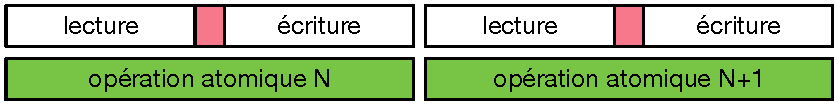
\includegraphics[scale=0.6]{./figures-pdf/time_atomic}
		\end{center}
	\end{block}  

\end{frame}
%%%%%%%%%%%%%%%%%%%%%%%%%%
\begin{frame}[plain, fragile]
\frametitle{Utilisation de la mémoire partagée}

\begin{lstlisting}[language=C]
__global__ void histo_kernel(unsigned char *in, long size, unsigned int *histo) 
{
  __shared__ unsigned int histo_private[NUMBRE_OF_BINS];
  
  if (threadIdx.x < NUMBRE_OF_BINS) {
    histo_private[threadidx.x] = 0;
  }
  __syncthreads();

  int i = threadIdx.x + blockIdx.x * blockDim.x;
  // stride is total number of threads
  int stride = blockDim.x * gridDim.x;
  
  while (i < size) {
    atomicAdd( &(private_histo[in[i] / NUMBRE_OF_BINS], 1);
    i += stride;
  }
     // wait for all other threads in the block to finish
  __syncthreads();

  if (threadIdx.x < NUMBRE_OF_BINS) {
          atomicAdd(&(histo[threadIdx.x]), private_histo[threadIdx.x] );
  }
}
 \end{lstlisting}
 
		\begin{center}
			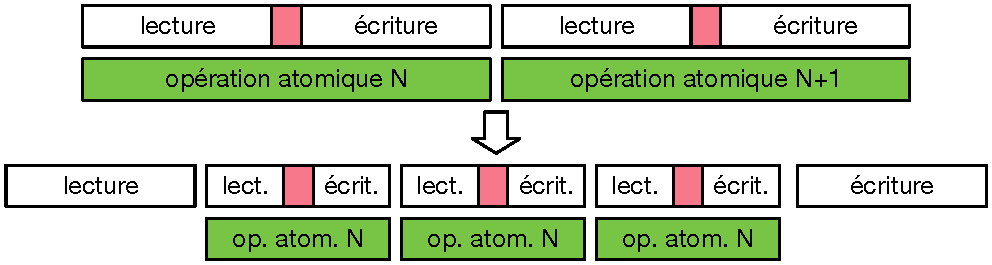
\includegraphics[scale=0.55]{./figures-pdf/optim}
		\end{center}
\end{frame}
%%%%%%%%%%%%%%%%%%%%%%%%%%

%%%%%%%%%%%%%%%%%%%%%%%%%%
\begin{frame}[plain]
\frametitle{Un peu de pratique avec le TD 10}

\begin{block}{Objectifs}
\begin{itemize}
	\item Utilisation d'opérations atomiques
	\item Utilisation d'une mémoire partagée
\end{itemize}
\end{block}
\end{frame}
%%%%%%%%%%%%%%%%%%%%%%%%%%
\end{document}